\subsection{Models}

\mysubsubsection{Sandra Beuck}{Gravitationsmaschine}

\begin{figure}[!htbp]%[htbp]
	\centering
		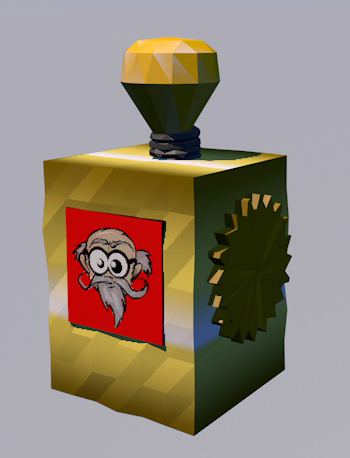
\includegraphics[width=0.8\textwidth]{images/gravinator}
	\caption{Gravitationsmaschine}
	\label{fig:gravinator}
\end{figure}

Die Gravitationsmaschine dient als Verbindungselement der Welten und ist in der Gebirgswelt prototypisch umgesetzt.

Sie ist eines der wichtigsten Elemente im Spiel, da sie in jeder Welt existent ist und somit ein Bezugspunkt für den Spieler darstellt. Aus diesem Grund ist die Gravitationsmaschine mit vielen Details, wie zum Beispiel einem Zahnrad, einem Bild des Wissenschaftlers und einer Kontrollleuchte versehen, und  erzeugt dadurch einen hohen Wiedererkennungswert. 

\mysubsubsection{Lydia Friedrich}{Remote Cube - Würfel}

\begin{figure}[!htbp]%[htbp]
	\centering
		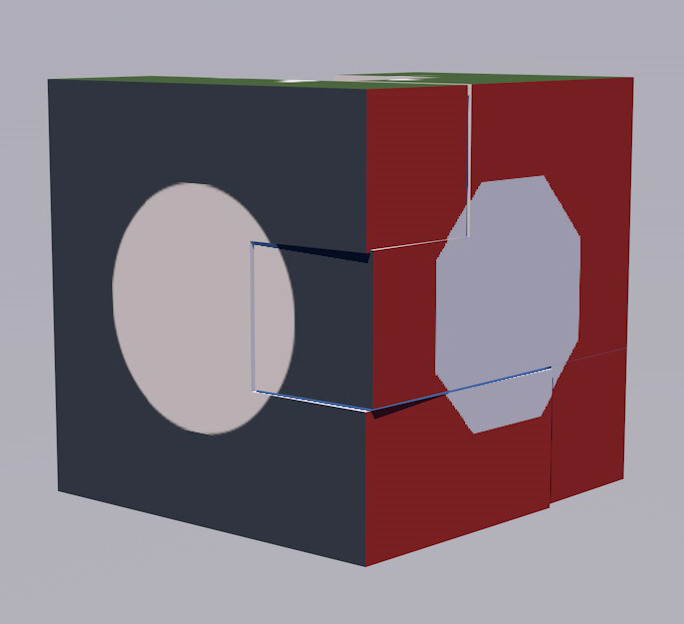
\includegraphics[width=0.8\textwidth]{images/RemoteCubeC4D}
	\caption{Virtueller Remote Cube}
	\label{fig:RemoteCube}
\end{figure}

Der Remote Cube ist die Verknüpfung des Würfels zur Außenwelt, denn nur mit ihm kann der Spieler das Spiel beenden und wieder in die reale Welt zurückkehren. Bevor dieses Ziel jedoch erreicht wird, müssen zunächst alle drei Teile des Remote Cubes erfolgreich vom Spieler eingesammelt werden (da der Remot Cube zu Beginn des Spiels zerbricht). Somit ist der Reomte Cube ebenfalls ein sehr wichtiges Spielelement da er das Symbol für den erfolgreichen Abschluß des Spiels darstellt.

Er ähnelt optisch dem Markerwürfel den der Spieler während des Spielens in den Händen hält und schafft so einen Bezug zwischen virtueller und realer Welt. Mit Hilfe von UV Mapping werden die Symbole des Markerwürfels auf den Remot Cube übertragen.